\center{
  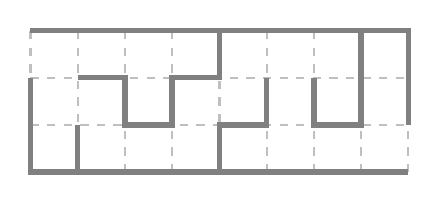
\begin{tikzpicture}[scale=0.6]
    \draw[thick, gray!50, dashed] (0,0) grid (8,3);
    \draw[line width=2, black!50]
      (0,2)--(0,0)--(8,0)
      (1,0)--(1,1)
      (0,3)--(0,3)--(4,3)--(4,2)--(3,2)--(3,1)--(2,1)--(2,2)--(1,2)
      (5,2)--(5,1)--(4,1)--(4,0)
      (8,1)--(8,3)--(0,3)
      (6,2)--(6,1)--(7,1)--(7,3)
    ;
  \end{tikzpicture}
  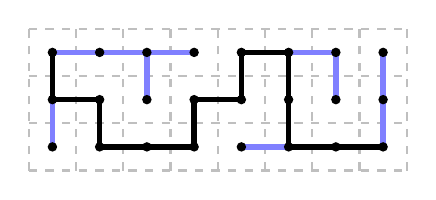
\begin{tikzpicture}[scale = 0.6]
    \draw[thick, gray!50, dashed] (0,4) grid (8,7);

    \draw[line width=2, blue!50]
      (7.5,4.5)--(7.5,6.5)
      (5.5,6.5)--(6.5,6.5)--(6.5,5.5)
      (5.5,4.5)--(4.5,4.5)
      (0.5,4.5)--(0.5,5.5)
      (0.5,6.5)--(3.5,6.5) (2.5,5.5)--(2.5,6.5)
    ;
    \draw[line width=2]
      (7.5,4.5)--(5.5,4.5)--(5.5,6.5)--(4.5,6.5)--(4.5,5.5)--(3.5,5.5)--
      (3.5,4.5)--(1.5,4.5)--(1.5,5.5)--(0.5,5.5)--(0.5,6.5)
    ;
    \foreach \x in {1,2,3} {
      \foreach \y in {0,1,...,7} {
        \fill (\y + 0.5, \x + 3.5) circle (0.1);
      }
    }
  \end{tikzpicture}
  }